\documentclass[tikz,border=10pt]{standalone}
\usepackage{amsmath}
\begin{document}
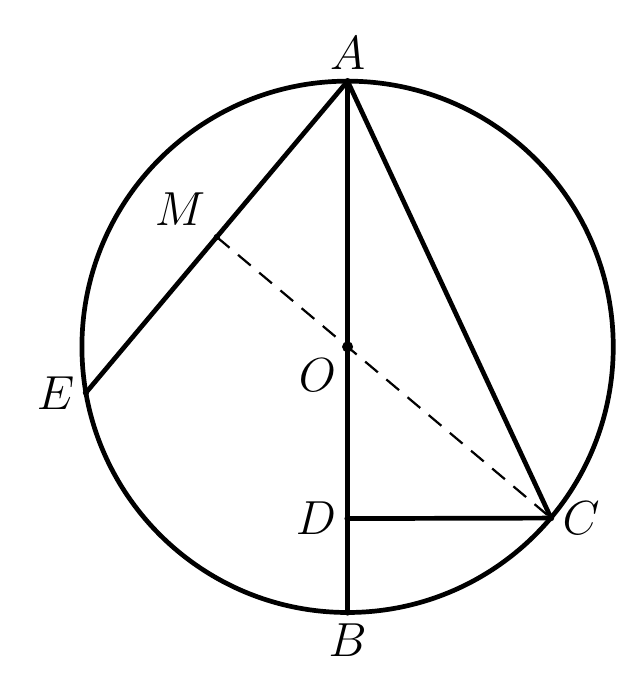
\begin{tikzpicture}[line join=round, line width=1.7pt]
  % Coordinates: scale s = 0.021448 cm/px, origin at O
  \coordinate (O) at (0,0);
  \coordinate (A) at (0,3.374);
  \coordinate (B) at (0,-3.374);
  \coordinate (C) at (2.584,-2.175);
  \coordinate (D) at (0,-2.181);
  \coordinate (E) at (-3.323,-0.583);
  % M moved to interior point on chord AE, on line M-O-C
  \coordinate (M) at (-1.661,1.394);

  % Circle
  \draw (O) circle (3.374);

  % Solid chord AB and lines AC, AE
  \draw (A) -- (B);
  \draw (A) -- (C);
  \draw (A) -- (E);

  % Dashed line from M through O to C (no overhang beyond M or C)
  \draw[dash pattern=on 6pt off 4pt, line width=0.8pt] (M) -- (O) -- (C);

  % Solid horizontal D to C
  \draw (D) -- (C);

  % Centre dot at O, drawn after all lines so it sits on top
  \fill[black] (O) circle (2pt);

  % Points
  \fill (A) circle (0.04);
  \fill (B) circle (0.04);
  \fill (C) circle (0.04);
  \fill (D) circle (0.04);
  \fill (E) circle (0.04);
  \fill (M) circle (0.04);

  % Labels
  \node[above] at (A) {\fontsize{17.5}{21}\selectfont $A$};
  \node[below] at (B) {\fontsize{17.5}{21}\selectfont $B$};
  \node[right] at (C) {\fontsize{17.5}{21}\selectfont $C$};
  \node[left] at (D) {\fontsize{17.5}{21}\selectfont $D$};
  \node[left] at (E) {\fontsize{17.5}{21}\selectfont $E$};
  % M label up-left of the point, inside the circle
  \node[above left] at (M) {\fontsize{17.5}{21}\selectfont $M$};
  \node[below left] at (O) {\fontsize{17.5}{21}\selectfont $O$};
\end{tikzpicture}
\end{document}